\label{chap:peening}

\epigraph{Since the early Middle Ages, mankind has always struggled to increase the hardness and flexibility of metals, to improve the durability and reliability of  metal tools and parts. From the Damascus steel smiths through the swordsmiths of medieval Japan, the method of cold-working metal by the application of precise mechanical pressure such as hammer blows has a glorious history.

In modern times, this concept has reached its apex with industrial surface hardening using shot peening, where thousands of small lead shots are fired at the metal surface, compressing and hardening the surface , improving the durability. With the advent of high power laser systems, an improved process has been developed, the process of laser shock peening.}{\textit{Samuel Zhrdne\\ HoloOr company}}


% because the paragraph alone leaves too much space
\section*{}

Laser shock peening (LSP) is a surface treatment process used to improve the mechanical performance (fatigue life, corrosion resistance, etc.) of metallic components. LSP induces residual stresses beneath the treated surface of metallic materials. These residual stresses are generated by high magnitude shock waves. A high magnitude of shock waves is achieved by the confined plasma generated at the metal surface by means of a high-intensity laser beam with a pulse duration in the tens of nanosecond range. Compared to traditional processes such as shot peening (SP), a LSP process can induce compressive residual stresses up to 1 mm in depth, which is approximately four times deeper than SP. LSP can be applied to various metallic components, such as:

\begin{itemize}
    \item aluminium alloys,
    \item titanium alloys,
    \item cast irons,
    \item nickel-based superalloys.
\end{itemize}

Firstly, this chapter deals with the physical and mechanical mechanisms of laser shock peening. Secondly, it focuses on the parameters of laser shock peening, namely:

\begin{itemize}
    
    \item laser power density,
    \item pulse shape and duration,
    \item laser wavelength,
    \item laser spot size and geometry,
    \item thermal protective coating, and confining overlay,
    \item coverage ratio of impacts \cite{dane_2000}.

\end{itemize}

 Lastly, this chapter describes the experimental equipment used for LSP at the HiLASE centre. 


\section{Laser shock peening overview}

\subsection{Laser shock peening process}
The configuration of an LSP process with a metallic component is shown in Figure~ \ref{fig:lspconfiguration}. An intense pulsed laser shock beam is focused onto a metal surface for a brief period of time (\SIrange{10}{100}{\ns}). The heated zone is vaporised and transformed to plasma by ionization due to high temperatures (over \SI{10000}{\degreeCelsius}). The plasma is under high pressure, which propagates through the material via shock waves. Two modes of LSP exist: 

\begin{itemize}

    \item direct ablation mode,
    \item confined ablation mode.

\end{itemize}

The direct ablation mode refers to the interaction of plasma with metal without coating and confinement \cite{sano}. Plasma pressure of tenths of a \SI{}{\GPa} is achieved using direct ablation mode. Higher pressures of \SIrange{1}{5}{\GPa} can be obtained using the confined mode. The confined ablation mode is known not only to increase the peak pressure of plasma by a factor up to ten, but also increases the duration of plasma by a factor of three in comparison with the direct ablation mode. In the confined mode, the metal surface is usually coated with an opaque material such as black paint or aluminium foil and confined by a material transparent to the laser radiation such as water or borosilicate glass. A stronger pressure pulse results in a higher magnitude of compressive residual stresses at a deeper depth \cite{fairland}. 

\begin{figure}[h]
    \centering
    
\includegraphics[width=0.6\linewidth]{img/lsp_configuration.jpg}
    \caption{Schematic configuration of laser shock peening process \cite{bohm_kaufman_brajer_rostohar_2019}}
    \label{fig:lspconfiguration}
\end{figure}

\subsection{Plasma, shock wave and residual stresses generation}

When the laser power density rises to several \SI{}{\giga\watt\per\cm\squared},  the surface of the material (or the absorbent coating -- if used) is heated and vaporised and forms plasma with pressure of several \SI{}{\giga\pascal} on the material's surface. The plasma absorbs the laser energy for the duration of the laser pulse. The plasma expands rapidly and generates a pressure pulse on the surface of the material.
As a consequence, a high-amplitude shock wave propagates through the material. When using the confined ablation mode with a transparent overlay, the plasma is held between the material and the transparent overlay, increasing the plasma's magnitude and amplitude. According to the above-mentioned description of the confined ablation mode, the LSP process can be regarded as a two-step method: 
\begin{enumerate}

    \item uniaxial compression of the irradiated area and dilation of the surface layer is caused by the rapid plasma expansion,
    
    \item the surrounding material reacts to this deformation and generates a compressive stress field.
    
\end{enumerate}

Before the reaction of the surrounding zones excluded from LSP, during the actual LSP process, uniaxial compression is induced in the direction of the shock wave propagation and a tensile state is induced in the plane parallel to the surface. 
After the reaction of the surrounding zones, a compressive stress field is generated in the affected zone, and a tensile stress field is created in the underlying layers of the material. 
The compressive stress field causes deformation in the material. The deformation is plastic as long as the peak dynamic stresses of the shock waves within the material are above the dynamic yield strength of the material. The process of compressive residual stress generation is shown in Figure \ref{fig:lspresidual} \cite{fabbro_peyre_berthe_scherpereel_1998}.



\begin{figure}[h]
    \centering
    
\includegraphics[width=0.6\linewidth]{img/residual_stress.jpg}
    \caption{Residual stresses formation with LSP:(a) stretching of impact area during interaction, (b) recovery of material after laser pulse has elapsed \cite{fabbro_peyre_berthe_scherpereel_1998}}
    \label{fig:lspresidual}
\end{figure}


The knowledge of the temporal and spatial profile of the confined plasma pressure provides insight into the optimisation of the LSP process. One of the simplest models for estimating plasma pressure was developed by Fabbro. It is based on the physical and mechanical behaviour of the laser-induced plasma and describes the LSP process in three steps:

\begin{enumerate}
    \item the laser pulse hits the material, and the confined plasma expansion causes shock waves to spread through the material,
    \item after the laser pulse has elapsed, the plasma cools down adiabatically, but the pressure is still present over a period approximately twice as long as the laser pulse duration,
    \item the adiabatic cooling continues, but the pressure of the plasma is already too low to drive shock waves deeper into the material.
\end{enumerate}

Assuming the plasma to be a perfect gas, the peak plasma pressure for water-confined ablation mode then holds:

\begin{gather} \label{pressure}
P(\SI{}{\giga\pascal}) = 0.01\sqrt{\frac{\alpha}{2\alpha + 3}}\sqrt{Z (\SI{}{\gram\per\cm\squared\per\second\squared})}\sqrt{I_{0} (\SI{}{\giga\watt\per\cm\squared})}
\end{gather} 

where:

\begin{itemize}
    \item $I_{0}$ -- laser power density,
    \item $\alpha$ -- efficiency of the interaction,
    \item $Z$ -- reduced shock impedance between the material and the confining medium
\end{itemize}
    
Based on Equation \ref{pressure}, we can assert that in the water-confined ablation mode, the peak pressure is directly proportional to the square root of the incident laser power density:

\begin{gather} \label{approx}
P(\SI{}{\giga\pascal}) \approx C\sqrt{I_{0} (\SI{}{\giga\watt\per\cm\squared})}
\end{gather} 

where:

\begin{itemize}
    \item $I_{0}$ -- laser power density,
    \item $C$ -- real constant \cite{fabbro_fournier_ballard_devaux_virmont_1990}.

\end{itemize}

\subsection{Transparent overlay and absorbent coating}

In the confined mode, the material is covered with two layers. The material surface is first coated with a nontransparent (absorption) overlay. The second layer is a transparent (confinement) overlay placed on the absorption layer.

The transparent overlay aims to prevent the laser-induced plasma from expanding freely from the metal surface.  The transparent overlay traps the expanding plasma on the metal surface. As a consequence, the plasma pressure rises higher than without the transparent overlay applied. Without the transparent overlay, the plasma would absorb the incident laser energy, but the laser energy would not be converted efficiently into a pressure pulse that induces compressive residual stresses in the material. The transparent overlay is placed on top of the absorbent coating. Any transparent material such as water, glass, fused quartz, and acrylic can be used as a transparent overlay, but a thin layer of water flowing over the coated surface is usually used because it is the easiest to apply \cite{clauer_lahrman_2001}.

The metal surface is usually laminated with a nontransparent material such as black paint, black vinyl tape, or aluminium foil. The absorption coating serves two purposes:

\begin{itemize}
    \item absorption coating -- increasing the absorption of the incident laser energy and thus increasing the shock wave intensity,
    \item thermal protective coating -- protecting the material surface from laser ablation and melting (the thermal effect is limited only to the protective coating) and thus preventing tensile strain from developing on the material's surface \cite{hong_wang_guo_wu_wang_dai_xia_xie_1998}.
\end{itemize}

\subsection{Laser shock peening overlapping strategy}

Overlapping of successive LSP processes (i.e., individual laser impact areas) is used to cover large areas with LSP. The coverage ratio is defined as the ratio between the overlapping area and the impact spot size for two successive LSP processes. An increase in the coverage ratio increases the plastically affected depth. Overlapping successive LSP processes results in a comparatively uniform distribution of compressive residual stresses across the overlapping regions.

During the peening process, a pattern is created made of individual laser pulses. Generally, multiple sequences of the pattern that are gradually shifted across the sample are used to create a layer, as seen in Figure \ref{fig:lspstrategy}. The pattern shifting ensures a more homogeneous residual stress distribution. This strategy's disadvantage is that the protective coating needs to be replaced in between sequences \cite{kaufman}.

\begin{figure}[h]
    \centering
    
\includegraphics[width=0.6\linewidth]{img/lsp_strategy.jpg}
    \caption{Laser shock peening strategy -- one layer consisting of four sequences \cite{bohm_kaufman_brajer_rostohar_2019}}
    \label{fig:lspstrategy}
\end{figure}



\subsection{Laser system parameters affecting the LSP process}

When performing a LSP process, the most challenging task is the choice of optimal LSP parameters (laser power density, laser spot size, absorbent coating) for the given material. If these parameters are chosen incorrectly, high tensile residual stresses can be induced on the material's surface, which can worsen the mechanical performance of the component \cite{clauer_holbrook_fairand_1981}.  

\subsubsection*{Laser system for laser shock peening overview}

Choosing an appropriate laser system is the first step in fulfilling the LSP process requirements. In LSP laser systems, the focus is mainly on the following parameters:
\begin{itemize}

    \item pulse energy: \SIrange{1}{100}{\joule}/pulse,
    \item pulse duration: $<$ \SI{100}{\nano\second},
    
    \item laser wavelength: three wavelengths are used for the LSP process most commonly:
    
    \begin{itemize}

        \item \SI{1064}{\nano\second} (near-infrared),
        \item \SI{532}{\nano\second} (green),
        \item \SI{355}{\nano\second} (ultraviolet).

    \end{itemize}
    
    \item sufficient repetition rate in the tens of hertz range.

\end{itemize}

The laser pulse energy influences the laser power density and therefore the magnitude of surface residual stress. 
The laser pulse duration and temporal shape affect the breakdown threshold of the laser power density. A shorter laser pulse with a short rise time usually results in a higher power density and higher peak pressure. 
The wavelength of the laser system influences the interaction between the laser pulse, absorption and confinement overlay and the material surface \cite{fabbro_peyre_berthe_scherpereel_1998}. 

\subsubsection*{Laser spot size and geometry}

One of the advantages of LSP is that the laser spot size and geometry can be adjusted to suit different applications. Laser spot sizes used for LSP vary between hundreds of micrometres and \SIrange{6}{10}{\mm} and usually have a round or square profile. The usable laser spot sizes are restricted mainly by the incident laser power density. The main difference between using a laser spot with a small diameter compared to a laser spot with a larger diameter lies in the way the shock waves expand in the material:

\begin{itemize}

    \item shock waves originating from a laser spot with a small diameter (\(r\)) expand like a sphere and attenuate at a rate of \(1/r^2\),

    \item shock waves originating from a laser spot with a larger diameter (\(r\))  expand like a planar front and attenuate at a rate of \(1/r\).

\end{itemize}

Consequently, the planar shock wave propagates further into the material, and the residual stresses reach deeper than the spherical shock wave \cite{bolger_montross_rode_1999}. 

The magnitude of residual stresses usually reaches its maximum at the surface and decreases with depth. This rule is valid for square laser spots. which minimalize the instability of the residual stresses at the centre of the laser spot. On the other hand, when using a circular laser spot, the residual stresses at the centre of the laser spot are unstable due to the complicated interactions of shock waves in this region \cite{masse_barreau_1995}. 

\subsubsection*{Laser power density and wavelength}

The magnitude of the laser power density plays a pivotal role in determining the magnitude of the plasma pressure. Moreover, the magnitude of the surface residual stresses is directly proportional to the magnitude of the plasma pressure. It is tempting to assume that by just increasing the laser power density, we will obtain higher surface stresses and thus a better quality LSP process. In reality, we are limited by several effects accompanying the laser-matter interaction:

\begin{itemize}

    \item dielectric breakdown of air can occur if the magnitude of the laser power density is too high. The dielectric breakdown is the generation of plasma not on the material surface, but in the area in front of it. This plasma absorbs the incoming laser pulse energy, thus limiting the energy to generate a shock wave in the material,

    \item when the magnitude of laser power density is higher than a certain threshold, the residual stresses increase in depth but decrease at the surface because of surface release waves,

    \item another consequence of increasing the laser power density above a certain threshold is the saturation and scattering of the corresponding pressure. The saturation of pressure is caused by the confining overlay breakdown phenomenon. The breakdown of the confining overlay has two negative consequences: 
    
    \begin{itemize}
        \item the pressure duration is shortened,
        \item the peak pressure is saturated.
    \end{itemize}
  
  
\end{itemize}    
As mentioned earlier, the three most commonly used wavelengths for LSP are near infrared, green, and ultraviolet. The near infrared wavelength has the highest absorption coefficient in the confining overlay and a high breakdown threshold. By contrast, the green overlay has the lowest absorption in the confining overlay and a lower breakdown threshold. The pressures produced by the laser pulses have similar profiles regardless regardless of the wavelength \cite{berthe_fabbro_peyre_bartnicki_1999}.



\subsubsection*{Laser pulse temporal profile and duration}

Laser systems with parameters suitable for LSP usually deliver two types of temporal shapes:

\begin{itemize}

    \item Gaussian,
    \item short rise time (SRT).
    
\end{itemize}

It was observed that SRT pulse shapes produce higher pressure on the metal surface and have a higher breakdown threshold than Gaussian pulse shapes. The pressure pulse duration is directly proportional to the laser pulse duration.  This fact is advantageous when it is possible to change the laser pulse duration of a laser system \cite{devaux_fabbro_tollier_bartnicki_1993}. 


\subsection{Laser shock peening applications}

Nowadays, LSP is heavily commercialized, and hundreds of patents regarding LSP have been issued. The industry leaders are General Electrics, LSP Technologies and Curtis Wright Surface Technologies. LSP is used in the following applications:

\begin{itemize}
 
    \item increase of fatigue life and fatigue strength of structures \cite{dane_hackel_daly_harrisson_2000},
    \item strengthening of thin sections \cite{vaccari_1992},
    \item hardening surfaces,
    \item shaping or straightening of parts  (laser peen forming).

\end{itemize}

LSP is expected to expand from current high-value, low volume parts to more mass-produced parts in the future, due to the steady advancements in laser systems suitable for LSP \cite{clauer_2019}. 



\section{Laser shock peening station and laser sources at HiLASE centre}

The HiLASE research centre is an infrastructure focused on laser research and development, located in Dolní Břežany, Czech Republic. HiLASE's Industrial laser applications program (ILA) focuses on LSP, laser induced damage threshold (LIDT), and laser micromachining technologies. ILA is equipped with several experimental stations, including an LSP station. 

The LSP station uses two laser sources:

\begin{itemize}
  \item Bivoj laser system,
  \item Litron LPY ST 7875-10 2HG laser.
\end{itemize}

 A laser beam distribution system (LBDS) distributes the beam from the laser laboratory located on the ground floor to the experimental laboratory located on the 1\textsuperscript{st} floor. The Bivoj laser system is a Diode Pumped Solid State Laser (DPSSL) based on Yb-doped gain media with a laser wavelength of 1030 nm capable of delivering energy pulses up to \SI{8}{\joule} at a \SI{10}{\hertz} repetition rate. The beam shape at the output of the Bivoj laser is a square flat-top pulse. An overview of the Bivoj laser system is shown in Figure \ref{fig:bivoj}. The two main sections of the Bivoj laser are the front-end and the \SI{10}{\joule} amplifier. The second laser source available at the LSP station is the Litron LPY ST 7875-10 2HG laser.
 
 \begin{figure}[h]
    \centering
    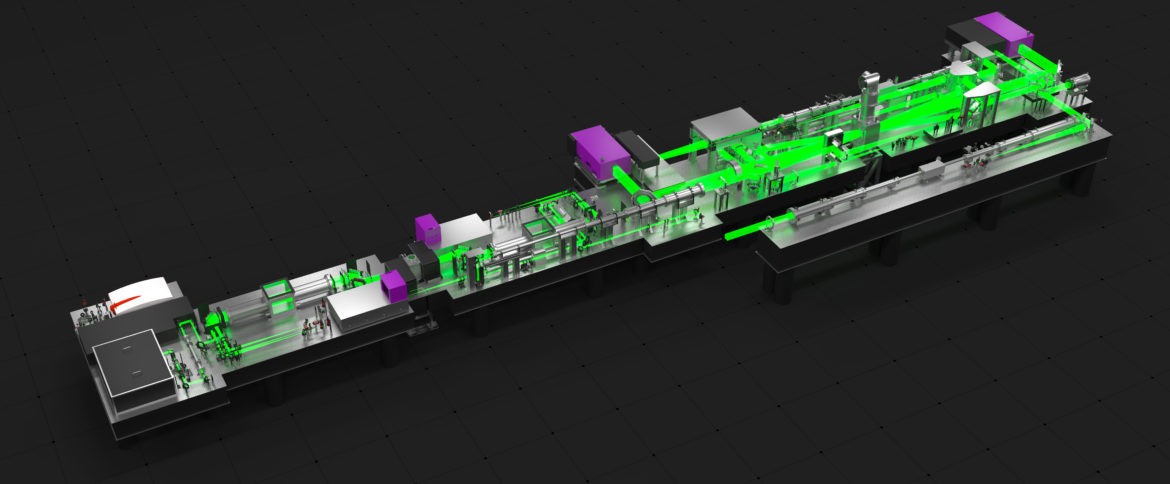
\includegraphics[width=1.0\linewidth]{img/bivoj.jpg}
    \caption{Laser system Bivoj: Diode-pumped solid-state (DPSSL) laser \cite{bivojiso}}
    \label{fig:bivoj}
\end{figure}
 
 \subsection{LSP station layout}
 \label{sec:lsp_layout}

The layout of the LSP station is shown in Figure \ref{fig:lsplayout}. The laser beam enters the LSP station through the LBDS output node and
continues to the optical table, where it is redirected and
focused on the target. The target itself is mounted on the
robotic arm. The laser beam position is fixed, so the robotic
arm needs to be moved to direct the laser to the sample.

\begin{figure}[h]
\centering
\begin{subfigure}{.45\textwidth}

    
\includegraphics[width=1\linewidth]{img/lsp_layout.jpg}

    \label{fig:a}
\end{subfigure}
\begin{subfigure}{.45\textwidth}

    \includegraphics[width=1\linewidth]{img/lsp_station_real.JPG}

    \label{fig:b}
\end{subfigure}

\caption{(Description of images from left to right) (1) schematic layout of LSP station, (2) photography of LSP station \cite{bohm_kaufman_brajer_rostohar_2019}}
\label{fig:lsplayout}
\end{figure}



\subsection{Bivoj laser system}

\subsubsection*{Bivoj front-end}

The front-end starts with a fibre-based section, consisting
of a fibre oscillator, a fibre amplifier, and a temporal pulse shaper
with \SI{125}{\ps} resolution. The output of the fibre front-end is fed
to the first booster amplifier, which is regenerative and
increases the energy to \SI{30}{\milli\joule} and reduces the repetition rate to \SI{10}{\hertz}. The second booster amplifier works in a multi-pass regime
and increases the pulse energy to approximately \SI{30}{\milli\joule}.
The repetition rate can be switched between \SI{1}{\hertz} and \SI{10}{\hertz}. The
beam shape at the front-end output is \SI{8 x 8}{\mm\squared} square flat top.

\subsubsection*{Bivoj 10 J amplifier}

The \SI{10}{\joule}  amplifier is the first-stage main amplifier based on
cryogenically cooled multislab technology. The principal
component of the amplifier is the amplifier head, where the
gain media are stored and cooled by gaseous helium to 
the temperature of about \SI{150}{\kelvin}. The laser beam from the front-end
is enlarged to \SI{22 x 22}{\mm\squared} and sent to the \SI{10}{\joule} amplifier, where
increases its pulse energy from approximately \SI{30}{\milli\joule} to
approximately \SI{8}{\joule} at \SI{10}{\hertz}. The spatial profile of the laser beam at the output of the Bivoj \SI{10}{\joule} amplifier is shown in Figure \ref{fig:spatialprofile} and the temporal profile is shown in Figure \ref{fig:temporalprofile} \cite{saumyabrata}.

\begin{figure}[h]
    \centering
    
\includegraphics[width=0.6\linewidth]{img/spatial_profile.jpg}
    \caption{Spatial profile of laser beam at output of Bivoj \SI{10}{\joule} amplifier and approximate dimensions \cite{kaufman}}
    \label{fig:spatialprofile}
\end{figure}

\begin{figure}[h]
    \centering
    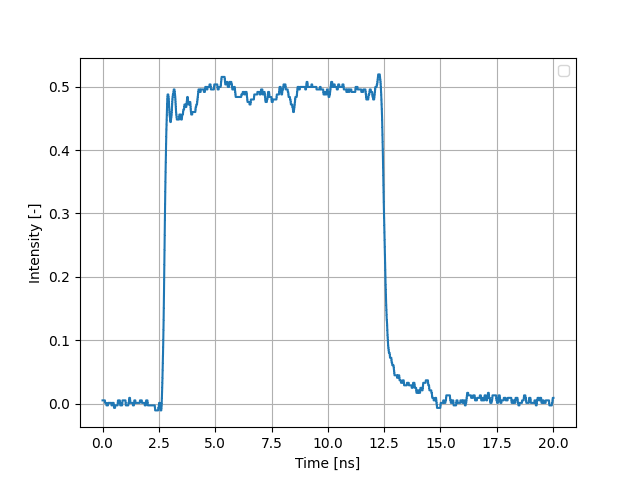
\includegraphics[width=0.6\linewidth]{img/bivoj_temp.png}
    \caption{Temporal profile of laser beam at output of Bivoj \SI{10}{\joule} \cite{kaufman}}
    \label{fig:temporalprofile}
\end{figure}

\subsection{Litron LPY ST 7875-10 2HG laser}

The second laser source available at the LSP station is the Litron LPY ST 7875-10 2HG laser, a tabletop laser located directly in the experimental laboratory next to the LSP station. This laser is a pulsed Q-switched Nd:YAG laser suited for industrial or research applications. The Litron  LPY ST 7875-10 2HG laser comes with a super-gaussian resonator. The most important parameters of this system are highlighted in Table \ref{tab:litronparameters} and the laser system is shown in Figure \ref{fig:litron} \cite{litron}. 


\begin{table}[h!] 
\centering
    \begin{threeparttable}
        \begin{tabular}{|c | c|} 
        \hline
            \textbf{Parameter} & \textbf{Value} \\ [0.5ex] 
        \hline
        Repetition Rate [Hz] & 10  \\ 
        \hline
            Output Energy [mJ] & \\
            1064nm & 3500 \\
            532nm & 1750 \\
        \hline
            Beam Diameter [mm] & 15 \tnote{a} \\
        \hline
            Beam Divergence [mrad] & <0.5 \tnote{b} \\ 
        \hline
            Pulse Length @1064nm [ns] & 10-12 \\
        \hline
            Pointing Stability [µrad] & 25 \tnote{c} \\
        \hline
            Timing Jitter [ns] & <0.5 \tnote{d}  \\
        \hline
        \end{tabular}
        \begin{tablenotes}
            \small
            \item[a] Peak-to-peak Energy -- 99 \% of pulses. 
            \item[b] Full angle for 90 \% of the energy.
            \item[c] Half angle.
            \item[d] Jitter is measured concerning the external Q-switch trigger input.
        \end{tablenotes}
        
    \end{threeparttable}
        \caption{Litron LPY ST 7875-10 2HG parameters \cite{litronmanual}}
\label{tab:litronparameters}
\end{table}

\begin{figure}[h]
    \centering
    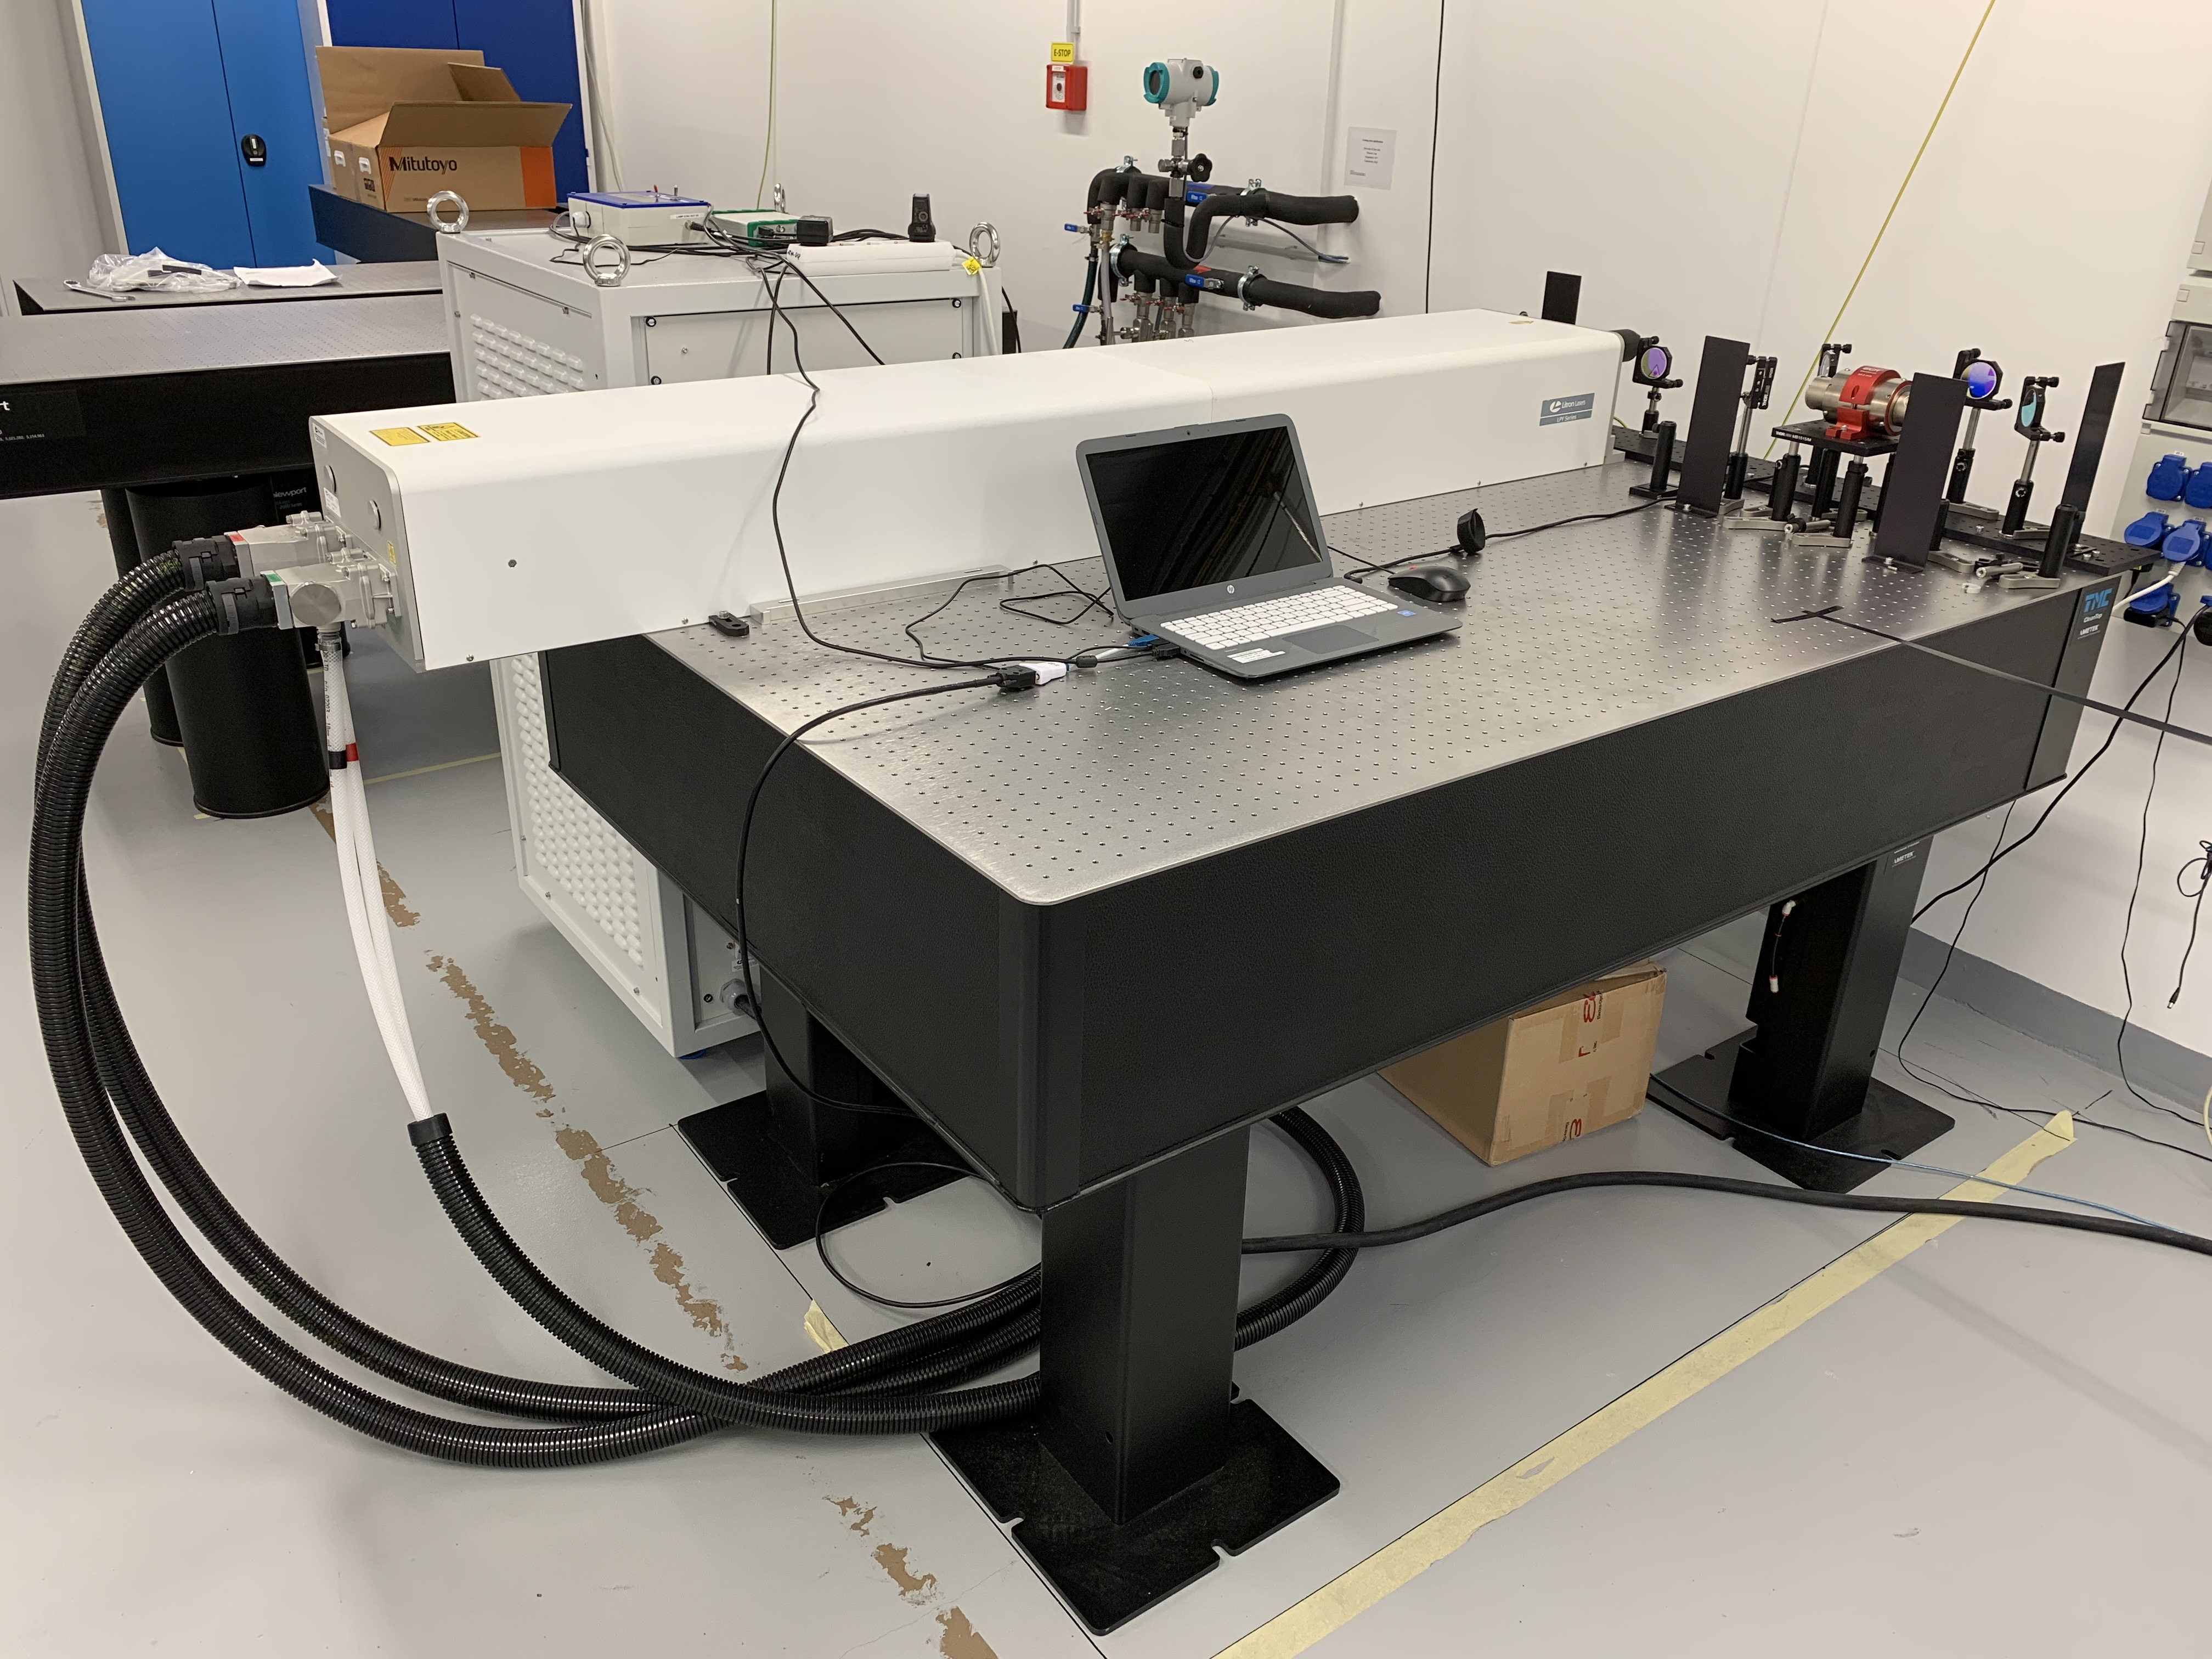
\includegraphics[width=0.6\linewidth]{img/litron.JPG}
    \caption{Litron LPY ST 7875-10 2HG laser at HiLASE centre}
    \label{fig:litron}
\end{figure}





\subsection{FANUC M-20iA/20M robotic arm}

The FANUC M-20iA/20M is a 6-axis universal industrial robotic arm with a maximum load capacity of \SI{20}{\kg} and a maximum reach of \SI{1811}{\mm}. The repeatability of the robotic arm is \SI{+-0.08}{\mm}. The FANUC M-20iA/20M is a multipurpose robotic arm and can be used for various applications such as assembling, packaging and machining \cite{fanucrobot}.

The robotic arm is coupled with a FANUC R-30iB controller. The R-30iB controller is equipped with a FANUC AIF01A PLC interface module. The interface module is connected to the following expansion modules:

\begin{itemize}
    \item AID16L -- 16 digital inputs,
    \item AOD16D -- 16 digital outputs,
    \item ADA02A -- 2 analog outputs. \cite{fanucunitmanual}
\end{itemize}

The FANUC AIF01A PLC interface module and its expansion modules are connected to the Bivoj and Litron lasers via digital inputs and outputs. In the case of the Bivoj laser system, the expansion modules are linked to a fast flipper located in the Bivoj laboratory. The fast flipper either redirects the laser beam into a cooled beam dump or lets it pass through the LBDS into the LSP station. The Litron laser is coupled to the robotic arm controller via an external trigger. 

\subsection{Electrical connection between FANUC R-30iB controller and Litron LPY ST 7875-10 2HG laser}

A block diagram of the electrical connection between FANUC R-30iB controller and Litron LPY ST 7875-10 2HG laser is shown in Figure \ref{fig:electronics}. The robotic arm PLC sends out a \textit{ROBOT GATE} digital output signal which acts as a gating signal for the \textit{EXTERNAL TRIGGER INPUT} signal. The \textit{EXTERNAL TRIGGER INPUT} signal is generated by the microcontroller unit (MCU). The \textit{LAMP SYNC OUTPUT} signal is fed back to the MCU and to the delay generator. The delay generator creates a delayed \textit{Q-SWITCH TRIGGER} signal which is inputed into the D/A  input of the laser controller. The \textit{Q-SWITCH TRIGGER} signal is delayed with respect to the \textit{LAMP SYNC OUTPUT} signal by $t_{QSW}$. The value of $t_{QSW}$ is fine-tuned with the help of the delay generator.  The timing diagram for internal triggering of the flashlamps and external triggering of the q-switch is shown in Figure \ref{fig:wave}, where:

\begin{itemize}
    \item $t_{BT}$ -- intra-cavity build up time (typically \SIrange{50}{100}{\ns}),
    \item $t_{QSW}$ -- timed by external electronics with respect to the external lamp trigger input (typically \SIrange{100}{500}{\us} for maximum output)

\end{itemize}


\begin{figure}[h]
    \centering
    
\includegraphics[width=1.0\linewidth]{img/electronics_3.jpg}
    \caption{Block diagram of the electrical connection between FANUC R-30iB controller and Litron LPY ST 7875-10 2HG laser}
    \label{fig:electronics}
\end{figure}

\begin{figure}[h]
    \centering
    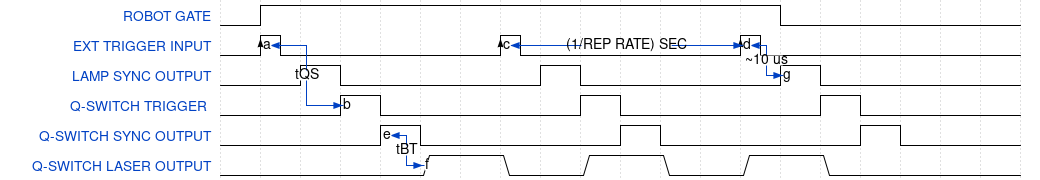
\includegraphics[width=1.0\linewidth]{img/wavedrom_bigger.png}
    \caption{Timing diagram for external triggering of flashlamp and internal triggering of the q-switch, where $t_{BT}$ is the intra-cavity build up time (typically \SIrange{50}{100}{\ns}) and $t_{QSW}$ is the internally timed q-switch delay (typically \SIrange{100}{500}{\us} for maximum output)}
    \label{fig:wave}
\end{figure}


The  FANUC M-20iA/20M robot and FANUC R-30iB controller are shown in Figure~ \ref{fig:robotcontroller} \cite{fanucrobotcontroller}. The electrical connection also allows to change the repetition rate of the laser (1 \SI{}{\hertz} or 10 \SI{}{\hertz}).



\begin{figure}[h]
\centering
\begin{subfigure}{.45\textwidth}

    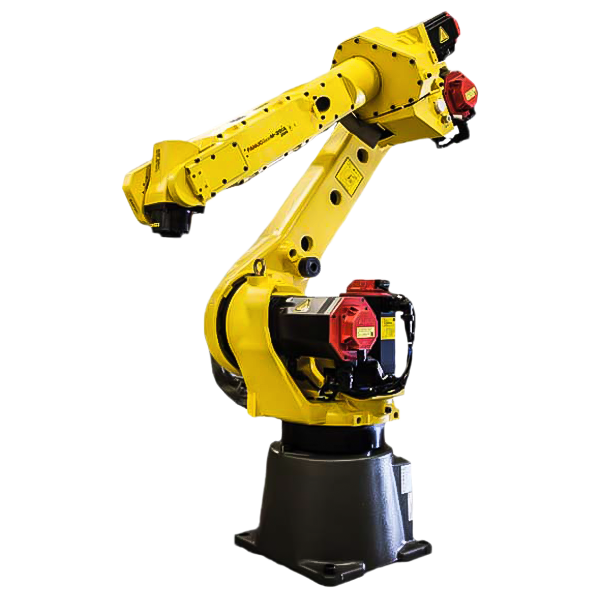
\includegraphics[width=1\linewidth]{img/fanuc_robot.png}

    \label{fig:a}
\end{subfigure}
\begin{subfigure}{.45\textwidth}

    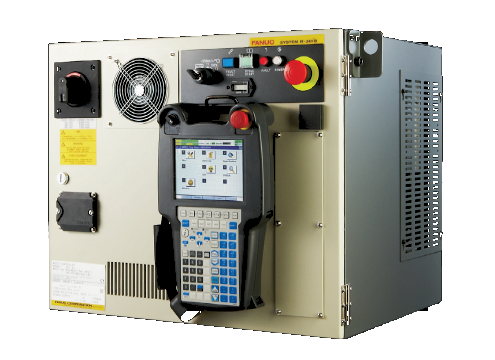
\includegraphics[width=1\linewidth]{img/fanuc_controller.png}

    \label{fig:b}
\end{subfigure}

\caption{(Description of images from left to right) (1) FANUC M-20iA/20M industrial robotic arm, (2) FANUC R-30iB controller with Teach Pendant \cite{fanucrobotcontroller}}
\label{fig:robotcontroller}
\end{figure}



\begin{comment}
\begin{figure}[h]
    \centering
    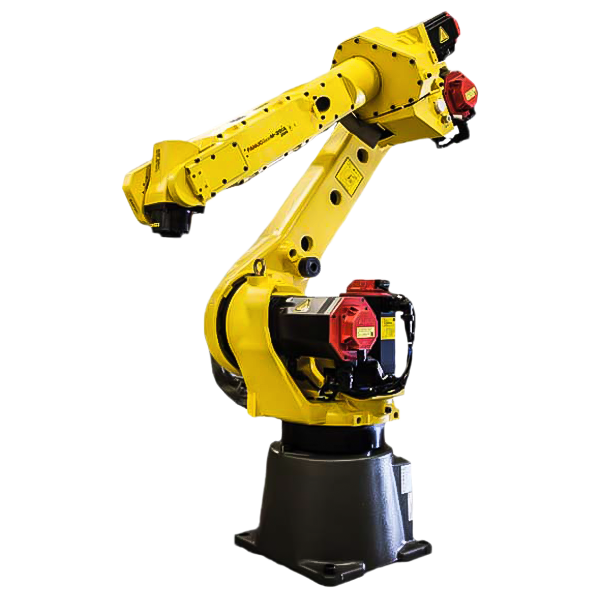
\includegraphics[width=0.6\linewidth]{img/fanuc_robot.png}
    \caption{FANUC M-20iA/20M industrial robotic arm  \cite{fanucrobot}.}
    \label{fig:fanucrobot}
\end{figure}
\end{comment}


\subsubsection*{Network connection of robot controller}


The robot controller must be reachable from the computer running the RoboDK application described in \hyperref[chap:design]{Chapter 3 -- Design}. In the LSP station, this is ensured by having the controllers and computer on the same local network as depicted in Figure \ref{fig:network}. 

\begin{figure}[h]
    \centering
    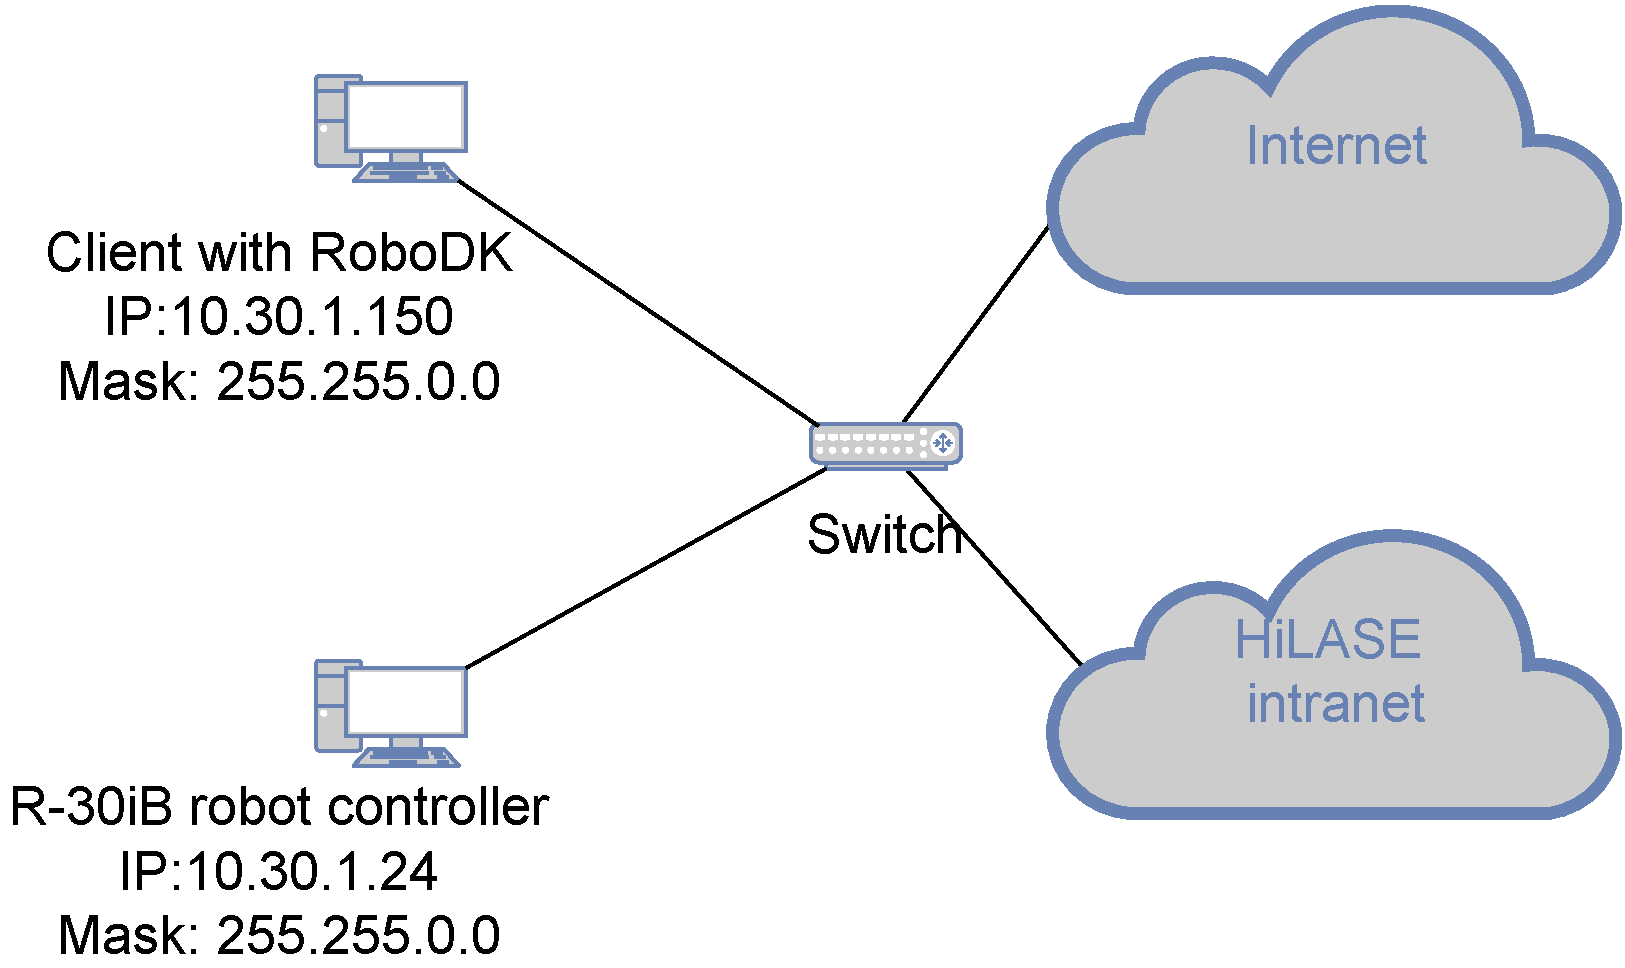
\includegraphics[width=0.8\linewidth]{img/network.pdf}
    \caption{Network diagram of the robotic arm workcell}
    \label{fig:network}
\end{figure}


\begin{comment}

\subsection{Network connection of robot controller}


The robot controller must be reachable from the computer running the RoboDK application described in \hyperref[chap:design]{Chapter 3 -- Design}. In the LSP station, this is ensured by having the controllers and computer on the same local network as depicted in Figure \ref{fig:network}. 

\begin{figure}[h]
    \centering
    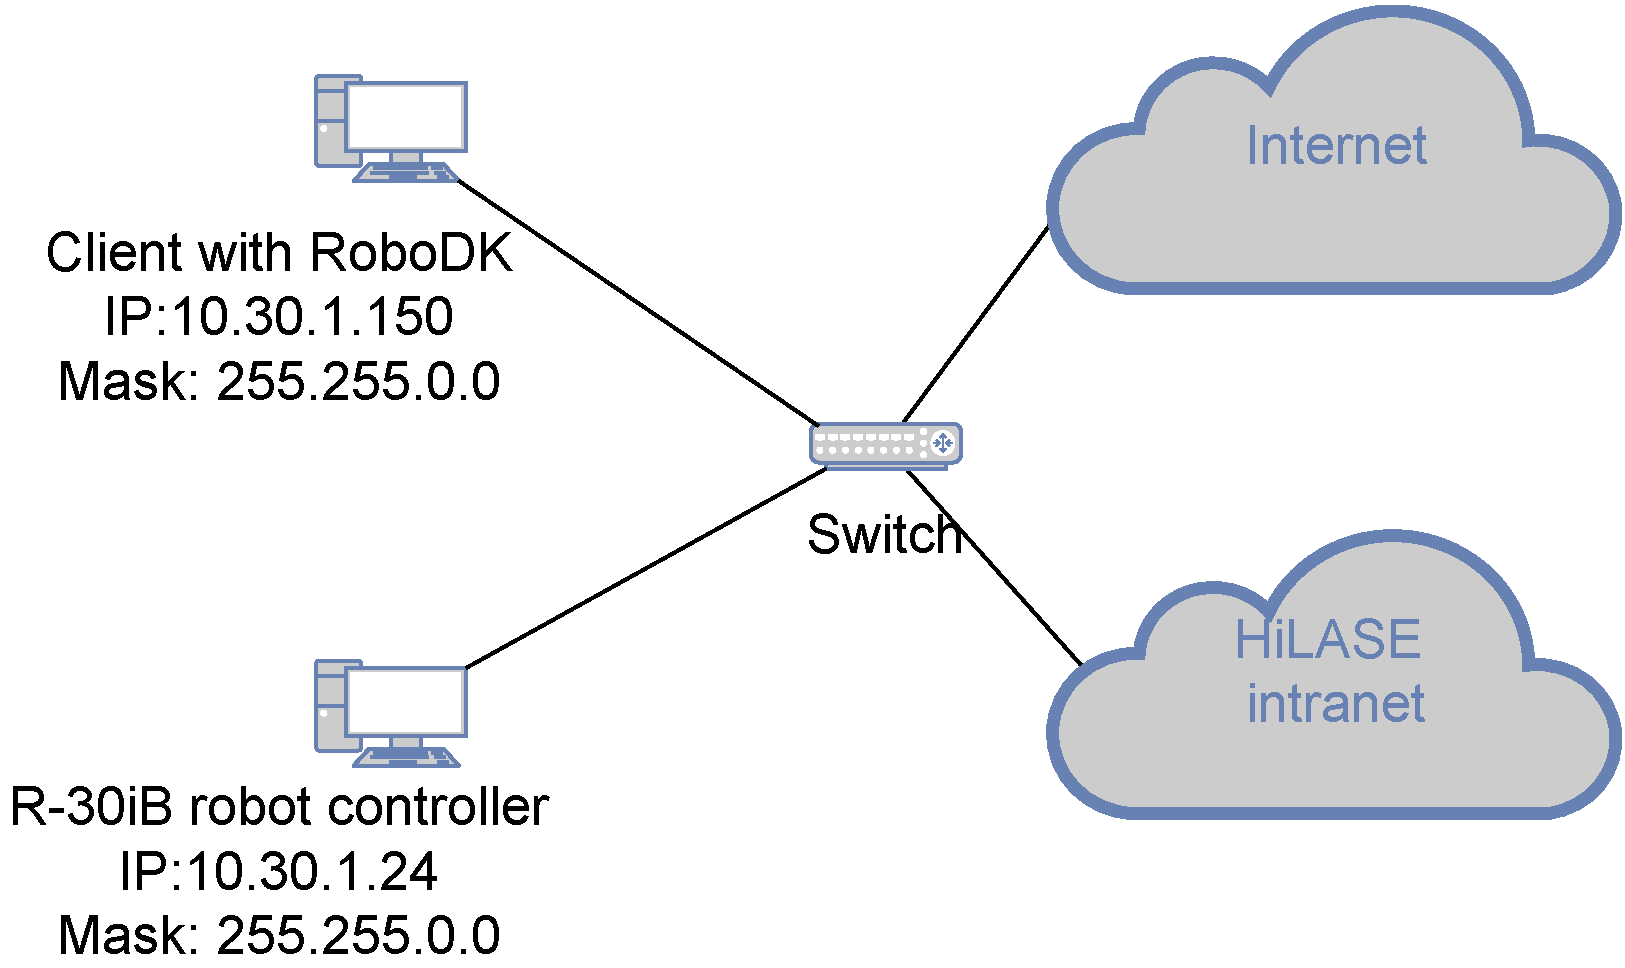
\includegraphics[width=0.8\linewidth]{img/network.pdf}
    \caption{Network diagram of the robotic arm workcell}
    \label{fig:network}
\end{figure}

\end{comment}

\subsection{LSP process example}

The following \href{https://www.youtube.com/watch?v=awhlLU91-dk&ab_channel=HiLASECentre}{video} shows the improvement of cavitation erosion resistance by LSP carried out at the HiLASE centre. This process is developed by HiLASE center and SIGMA GROUP Plc. for the improvement of cavitation erosion resistance of pump blades. The parameters chosen for this experiment are shown in Table \ref{experimentalparameters}. 

\begin{table}[h!]
\centering
    \begin{threeparttable}
        \begin{tabular}{|c | c|} 
        \hline
            \textbf{Parameter} & \textbf{Value} \\ [0.5ex] 
        \hline
        Laser source & Bivoj laser system  \\
        \hline
        Wavelength [\SI{}{\nano\second}] & 1030 \\
        \hline
        Repetition Rate [\SI{}{\hertz}] & 10  \\ 
        \hline
            Pulse energy at sample [\SI{}{\milli\joule}] & 5000 \\
        \hline
            Beam size at sample [\SI{}{\mm\squared}] & 4 \\
        \hline
            Pulse Length @1030nm [\SI{}{\nano\second}] & 10 \\
        \hline
            Power density at sample [\SI{}{\giga\watt\per\cm\squared}] & 5.56 \\

        \hline
        \end{tabular}

        \caption{Experimental parameters of laser shock peening for improvement of cavitation erosion resistance}
        \label{experimentalparameters}
    \end{threeparttable}
\end{table}

